\chapter{Projeção de operacionalização, governança e avaliação econômica}
Este capítulo formula um cenário de uso futuro. As listas, categorias, escores e consultas retrospectivas foram produzidas computacionalmente; revisão humana, despacho, registro de OS/TOI, encerramento e realimentação são etapas propostas, não funções de campo avaliadas.
\section{Ciclo do caso, filas e capacidade}
A implantação proposta submete os indícios a revisão humana e distingue três destinos: qualidade de dados e telecomunicação, investigação técnica da instalação ou rede e avaliação comercial de casos elegíveis. O registro da decisão conservaria o corte, a versão do modelo e a evidência disponível naquele instante. Uma UC poderia permanecer em observação, avançar para análise, ter o episódio encerrado ou ser reaberta após nova ocorrência. O identificador do episódio permite distinguir persistência diária de incidência.

A Figura \ref{episodios} apresenta os destinos propostos para a triagem e o registro comum ao encerramento das decisões.

\begin{figure}[htbp]\centering\caption{Fluxo proposto de triagem por episódio e registro da decisão técnica}\label{episodios}
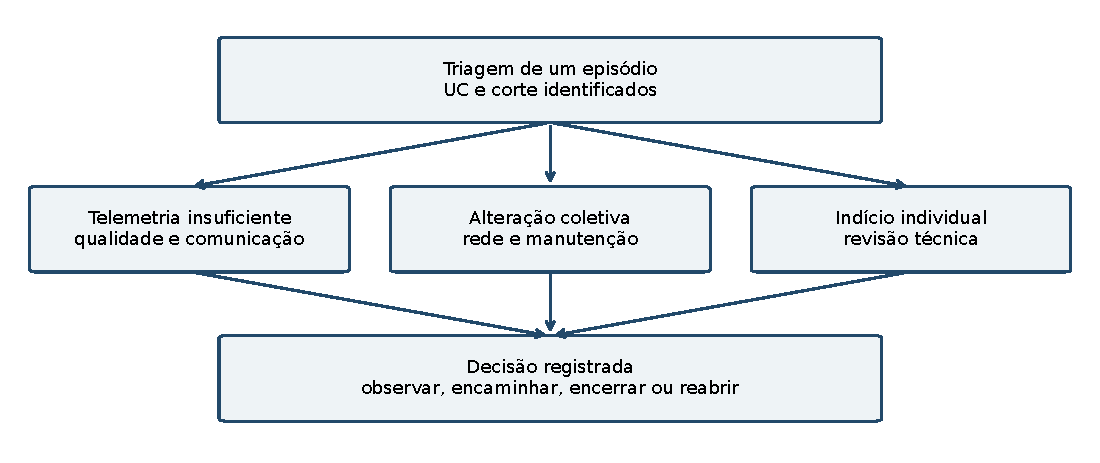
\includegraphics[width=0.96\textwidth,height=0.46\textheight,keepaspectratio]{figuras/episodios.pdf}
\par\small Fonte: elaboração própria.
\end{figure}
Adotou-se o mês $n$ como período da projeção. $B_n$ representa o estoque ao início do mês, $A_n$ as entradas únicas de episódios, $R_n$ as conclusões efetivas que consomem capacidade de inspeção, $X_n$ as baixas administrativas sem inspeção e $K_n$ a capacidade mensal. $R_n$ e $X_n$ são conjuntos disjuntos de baixas. A Equação \eqref{backlog} conserva o estoque e impede baixas superiores à demanda. Uma saída da lista diária só altera o estoque de episódios se houver decisão explícita de encerramento.

\begin{equation}\label{backlog}
B_{n+1}=B_n+A_n-R_n-X_n,\quad 0\leq R_n\leq K_n,\quad R_n+X_n\leq B_n+A_n
\end{equation}
Para capacidade positiva, a razão entre estoque acrescido de entradas e capacidade descreve a pressão bruta de atendimento. Valores acima da unidade indicam que o conjunto excede as vagas disponíveis naquele período. A seleção pode considerar persistência, qualidade e convergência de indícios. O aumento de rigor também altera as classes e os circuitos que obtêm acesso à revisão e deve permanecer rastreável.

\section{Reserva de capacidade e comparação com a carteira vigente}
A hipótese de planejamento admitiu 2.000 vagas mensais e reserva de até 40\% aos candidatos externos à lista vigente. Para $D_{\mathrm{novo},n}$ igual ao número de episódios externos que atingiram o critério mínimo, a Equação \eqref{reserva} limita a reserva à demanda qualificada e preserva vagas inteiras. Nesse cenário, o teto de novas indicações é 800 e a carteira convencional conserva pelo menos 1.200 vagas. A política depende de capacidade real, de acesso à lista convencional e de aprovação operacional.

\begin{equation}\label{reserva}
K_{\mathrm{novo},n}=\min(D_{\mathrm{novo},n},\lfloor0{,}40K_n\rfloor),\quad K_{\mathrm{legado},n}=K_n-K_{\mathrm{novo},n}
\end{equation}
\begin{table}[htbp]\centering\small\caption{Coortes propostas para avaliação prospectiva da carteira}\label{coortes}
\begin{tabular}{>{\raggedright\arraybackslash}p{\dimexpr 0.19\linewidth-2\tabcolsep\relax}>{\raggedright\arraybackslash}p{\dimexpr 0.44\linewidth-2\tabcolsep\relax}>{\raggedright\arraybackslash}p{\dimexpr 0.37\linewidth-2\tabcolsep\relax}}\toprule
Coorte & Regra temporal & Grandeza de interesse \\ \midrule
O — sobreposição & A UC já integrava a lista convencional no instante da decisão & Efeito da reordenação sobre o rendimento inicial \\
A — antecipação & A UC externa entrou posteriormente na lista convencional dentro do horizonte & Antecedência entre decisões comparáveis \\
N — descoberta incremental & A UC permaneceu externa até o fim do horizonte e obteve confirmação independente & Positivos adicionais e custo de oportunidade \\
\bottomrule\end{tabular}
\par\small Fonte: elaboração própria a partir dos dados e métodos do estudo.
\end{table}
A classificação da Tabela \ref{coortes} exige fixar o horizonte previamente. Uma UC externa ainda em acompanhamento permanece com classificação aberta. A comparação deve resguardar a carteira convencional tal como existia na data da decisão. Consultar apenas sua versão posterior incorporaria informações indisponíveis no momento da triagem.

\section{Indicadores prospectivos e custo de oportunidade}
Se os primeiros k casos inspecionados tiverem desfecho conclusivo, y indica confirmação independente e a Equação \eqref{yield} define o rendimento à profundidade k e o lift em relação à ordenação convencional. K indica capacidade e k indica profundidade efetivamente avaliada. Casos pendentes, inconclusivos ou não executados exigem contagem própria. Com acompanhamento incompleto, devem-se informar o denominador conclusivo e sua cobertura entre os selecionados. O lift exige rendimento convencional positivo.

\begin{equation}\label{yield}
\mathrm{Yield}@k=\frac{1}{k}\sum_{j=1}^{k}y_{(j)},\qquad \mathrm{Lift}@k=\frac{\mathrm{Yield}_{\mathrm{modelo}}@k}{\mathrm{Yield}_{\mathrm{base}}@k}
\end{equation}
Para uma UC i presente nas duas políticas com datas comparáveis, a Equação \eqref{tempo} define a antecedência. O valor positivo corresponde à decisão antecipada pelo modelo. Um desfecho ainda não observado até o fim do horizonte é censurado. A hipótese original de aumento de cinco pontos percentuais no rendimento ($\Delta Y = 0{,}05$) constitui meta de projeto sujeita à pactuação em piloto e depende do denominador adotado: se medido sobre a política mensal completa ($K = 2.000$), corresponde a $\Delta N = K\,\Delta Y = 100$ vistorias positivas adicionais; se medido exclusivamente sobre as $K_{\mathrm{novo},n} \le 0{,}40 K_n = 800$ vagas reservadas ao modelo, corresponde a $\Delta N = K_{\mathrm{novo},n}\,\Delta Y = 40$ vistorias.

\begin{equation}\label{tempo}
\Delta t_i=t_{\mathrm{base},i}-t_{\mathrm{modelo},i}
\end{equation}
O valor esperado de uma inspeção depende da probabilidade de confirmação p, da fração efetivamente realizável \ensuremath{\theta}, do valor potencial V e do custo C. A Equação \eqref{valor} explicita o custo de substituir uma inspeção convencional j por uma indicação i. Os parâmetros dependem de resultados independentes, custos observados e distinção entre cobrança pleiteada e valor recebido.

\begin{equation}\label{valor}
\mathrm{EMV}_i=p_i\theta_iV_i-C_i,\qquad \Delta\mathrm{EMV}_{i\leftarrow j}=\mathrm{EMV}_i-\mathrm{EMV}^{\mathrm{base}}_j
\end{equation}
Em um exercício de sensibilidade separado — dimensionado sobre as 274 UCs marcadas como candidatas à vistoria no consolidado exploratório de 66.099 unidades (em contraste com o teto mensal de $K=2.000$ vagas do cenário anterior) — adotaram-se custo unitário de R\$ 180, valor potencial de R\$ 1.800 e realização de 65\%. Com probabilidade assumida de 15\%, o custo total seria de R\$ 49.320 e o valor bruto esperado, de R\$ 48.087. O saldo seria negativo em R\$ 1.233. Ao elevar apenas a probabilidade assumida para 25\%, o saldo passaria a R\$ 30.825. O ponto de equilíbrio do exercício é $p^*=C/(\theta V)=180/(0{,}65\times 1800)\approx 15{,}38\%$. O exercício revela a dependência do resultado das hipóteses econômicas e mantém sua carteira hipotética separada do funil OOT.

\section{Protocolo de verificação e governança}
Uma avaliação prospectiva registraria população elegível, lista ordenada, posição, versão dos parâmetros, regra acionada e vínculo com a lista convencional antes da decisão. A revisão técnica documentaria encaminhamento ou abstenção, motivo e data. A apuração posterior classificaria desfechos conclusivos positivos, negativos, inconclusivos e não executados, preservando o acesso restrito ao vínculo com a UC.

A comparação entre políticas requer orçamento, período e critério de confirmação comuns. A seleção exclusiva dos casos mais bem pontuados impede estimar desempenho na parcela restante. Uma amostra de comparação e a estratificação por alimentador, cobertura e classe permitem examinar esse viés. Para casos inconclusivos, o acompanhamento deve distinguir tempo de espera de resultado negativo. Recalibração, alteração de peso e promoção de versões devem conservar a referência anterior e o histórico de decisões.


No cenário hipotético de 2.000 inspeções por mês, os estoques pontuais de 6.037 e 4.311 candidatos correspondem a 3,02 e 2,16 vezes a capacidade mensal. Essas razões não representam meses necessários para eliminar a carteira: a demanda recorrente exige deduplicação por episódio e registro das conclusões efetivas.


